Quelltexte können in zwei verschiedenen Kontexten in Fragestellungen auftauchen: Einerseits gibt es unvollständige, kurze Quelltext-Fragmente, die in einen Fließtext eingebunden werden sollen, beispielsweise:

\begin{center}
„Wie viele String-Parameter hat die folgende Java-Methode?\newline
public String m(int i, int s, boolean b) \{ ... \}“
\end{center}

Dabei handelt es sich nicht um ein syntaktisch nicht vollständiges und nicht-ausführbares Fragment. Um die Lesbarkeit dieses Fragments zu erhöhen, sollte es trotzdem optisch deutlich vom Fließtext unterscheidbar sein. Es bietet sich an, den Code in einer Monospace-Schriftart zu formatieren und ggf. Syntax-Highlighting anzuwenden.

\begin{figure}[H]
    \centering
    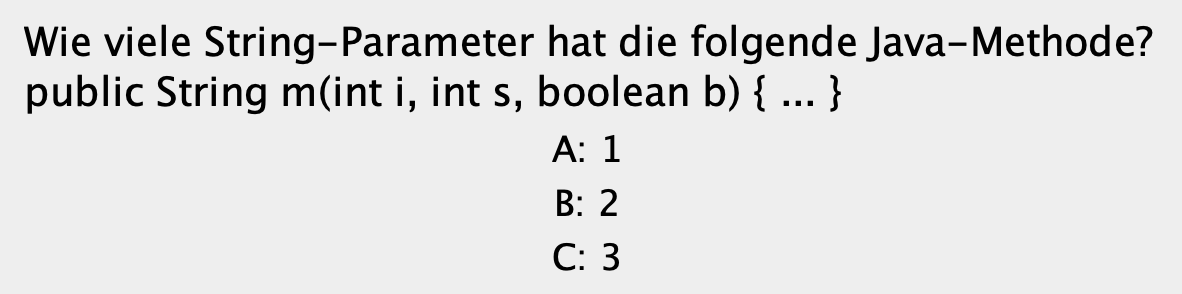
\includegraphics[width=\textwidth,frame]{chapter/entwurf/bilder/sturesy_fragment.png}
    \caption{Darstellung eines Code-Fragments in StuReSy (ohne manuelle Formatierungen)}
    \label{abb:sturesy_code_fragment}
\end{figure}


\begin{figure}[H]
    \centering
    \fbox{
    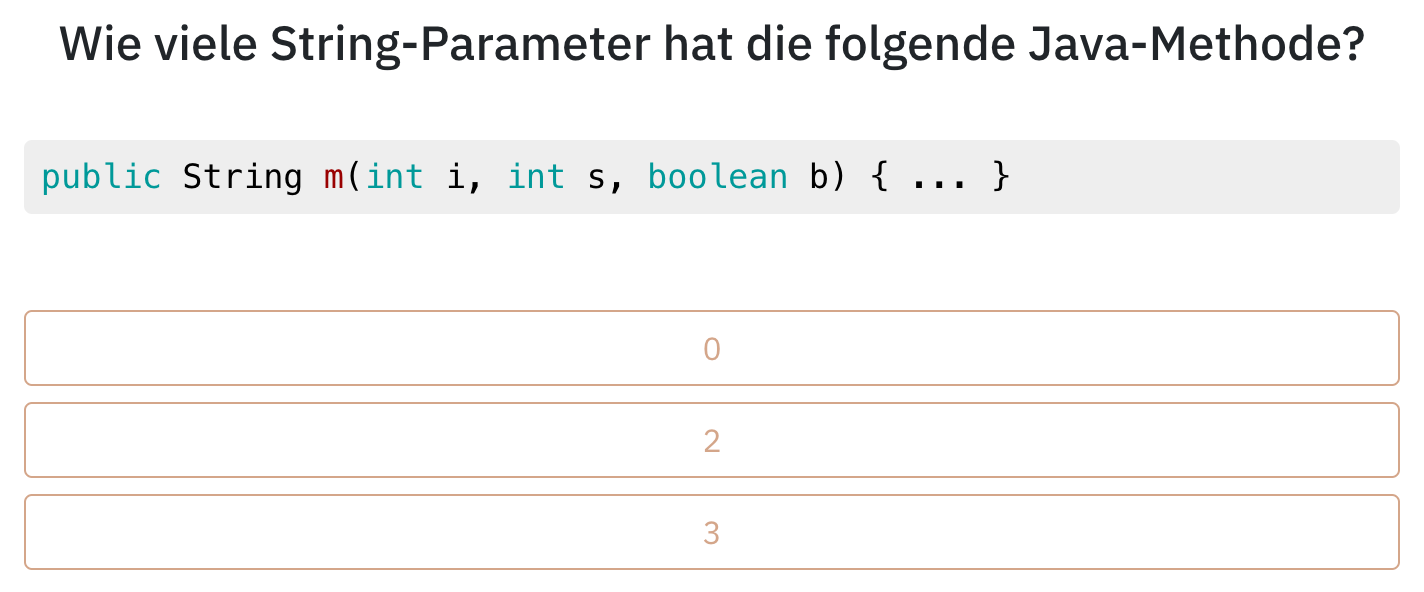
\includegraphics[width=\textwidth]{chapter/entwurf/bilder/weclare_fragment.png}
    }
    \caption{Darstellung eines Code-Fragments in Weclare (automatische Formatierung)}
    \label{abb:weclare_code_fragment}
\end{figure}

Der zweite Kontext von Quelltext in Fragestellungen ist vollständiger, ausführbarer Code

Um Fragestellungen mit Text-Formatierungen zu versehen ist eine simple Editor-Komponente notwendig, die mit einer grafischen Benutzeroberfläche ausgestattet ist. Eine solche Komponente selber zu implementieren ist sehr aufwendig, außerdem gibt es in diesem Segment bereits viele existierende Lösungen in der JavaScript-Landschaft. So wurden verschiedene Bibliotheken getestet und in Erwägung gezogen: Draft.js, CodeMirror, Slate, Prosemirror, Quill.

Letztendlich muss eine Editor-Komponente in diesem Projekt folgende Anforderungen erfüllen:

\begin{itemize}
    \item Integrierbarkeit mit React
    \item Möglichkeit um Syntax-Highlighting zu realisieren
    \item Simple Text-Formatierungen (Fett, Kursiv, etc)
\end{itemize}

Der Quill-Editor erfüllt alle diese Kriterien und wurde deswegen